\textbf{Ejecute el circuito generado mediante las siguientes instrucciones:}\vspace{.2cm}

\begin{minted}[fontsize=\small, linenos, frame=single]{python}
circuito2 = QuantumCircuit(1)

circuito2.h(0)
circuito2.z(0)
circuito2.h(0)

circuito2.barrier(0)

circuito2.h(0)

circuito2.measure_all()

circuito2.draw('mpl')
\end{minted}

\begin{center}
    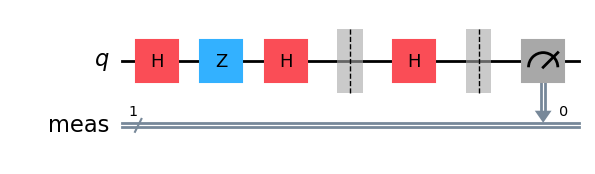
\includegraphics[height=3.5cm]{src/Img/2.png}
\end{center}

Que nos genera el siguiente histograma: 

\begin{center}
    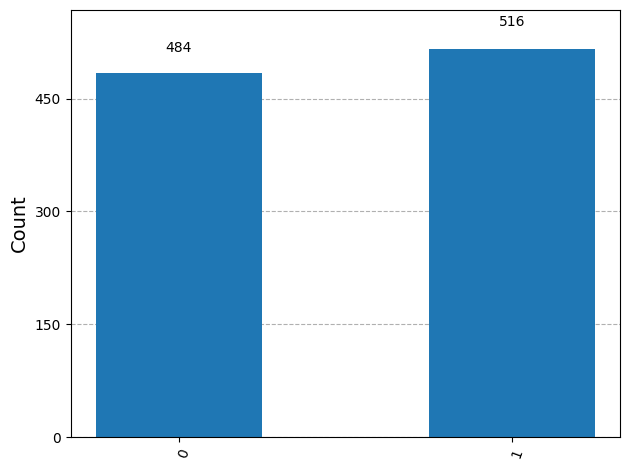
\includegraphics[height=6cm]{src/Img/2.1.png}
\end{center}

\textbf{A partir del histograma, ¿puede determinar el estado final del sistema? Si no es posible, ¿cómo podría solucionarlo?} \vspace{.2cm}

\begin{quote}
    Únicamente usando el histograma no nos es posible determinar con exactitud el estado final
    del sistema pues se encuentra en superposición, podemos decir que por la cantidad tan
    cercana a .5 se trata del estado $\ket{+}$ o $\ket{-}$, sin embargo, para saberlo con
    exactitud podemos operar matemáticamente con las compuertas o usar código. Veámoslo, con
    compuertas primero notar que la compuerta $\hat{H}$ aplicada 2 veces seguida es la
    identidad por lo que podemos de hecho ignorar estas ultimas 2. Lo siguiente es que
    sabemos que nuestro qubit se inicializa en $\ket{0}$ por defecto, por lo que al aplicar
    la primera compuerta tenemos que $\hat{H}\ket{0}=\ket{+}$ y Z hace cambio de fase lo que
    nos lleva a $\ket{-}$. También se puede utilizar una compuerta $\hat{H}$ sobre el
    resultado antes de medir para obtener un 1 y saber que en efecto se trataba de dicha
    compuerta. Las imágenes del histograma y el circuito están aquí:

    \begin{center}
        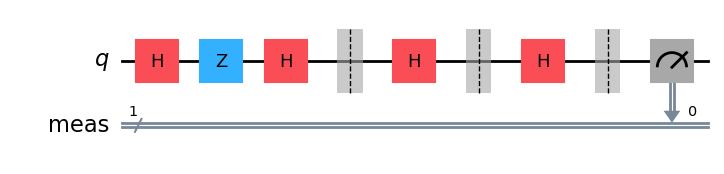
\includegraphics[height=3.5cm]{src/Img/2.3.png}
    \end{center}

    \begin{center}
        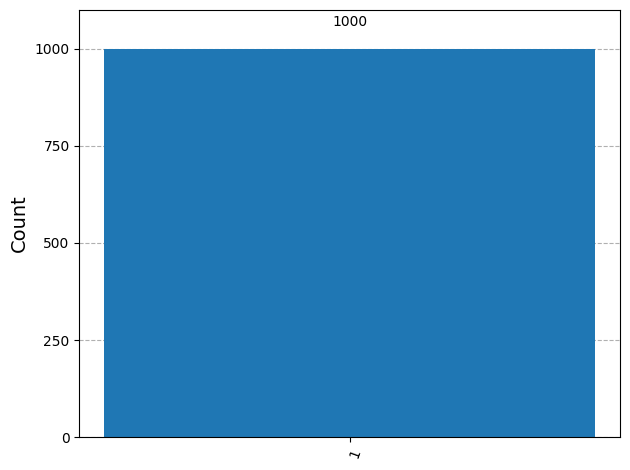
\includegraphics[height=6cm]{src/Img/2.4.png}
    \end{center}
\end{quote}
